
\documentclass[preview, tikz]{standalone}


% default packages
\usepackage{amsmath,amsfonts,amssymb,enumitem,mathtools}


\usepackage{tikz}
\usepackage{tikz-qtree}

\begin{document}

\begin{center}
    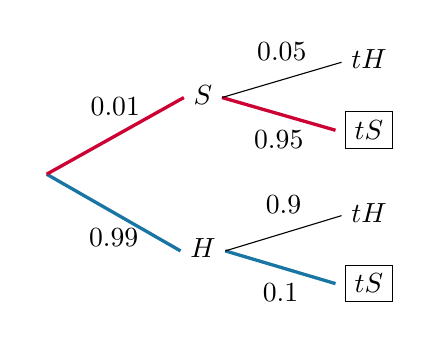
\begin{tikzpicture}[grow=right]
\tikzset{level distance=60pt,sibling distance=5pt}
\tikzset{execute at begin node=\strut}
\Tree [.{}
    \edge[very thick, draw=blue!60!green!90]  node[below] {$0.99$};
    [.$H$
        \edge[very thick, draw=blue!60!green!90] node[below] {$0.1$};
        $\boxed{tS}$
        \edge node[above] {$0.9$}; $tH$
    ]
    \edge[very thick, draw=red!80!blue] node[above]{$0.01$};
    [.$S$ 
        \edge[very thick, draw=red!80!blue] node[below]{$0.95$};
        $\boxed{tS}$ 
        \edge node[above]{$0.05$}; $tH$ 
    ]
]
\end{tikzpicture}
\end{center}
\end{document}